\section{Tiền xử lý số liệu}
\subsection{Đọc dữ liệu}
Trước hết, ta sẽ đọc dữ liệu từ tệp tin ``dirty\_data.csv'' bằng hàm \textbf{read.csv()}. Sau đó, ta sẽ tiến hành quan sát 5 dòng đầu tiên trong bảng dữ liệu được thể hiện trong hình \ref{fig:3.1}. Ngoài ra, hình \ref{fig:3.2} biểu diễn các cấu trúc dữ liệu ban đầu của các biến trong dữ liệu gốc bằng cách sử dụng hàm \textbf{str()}.
\begin{figure}[!htbp]
    \centering
    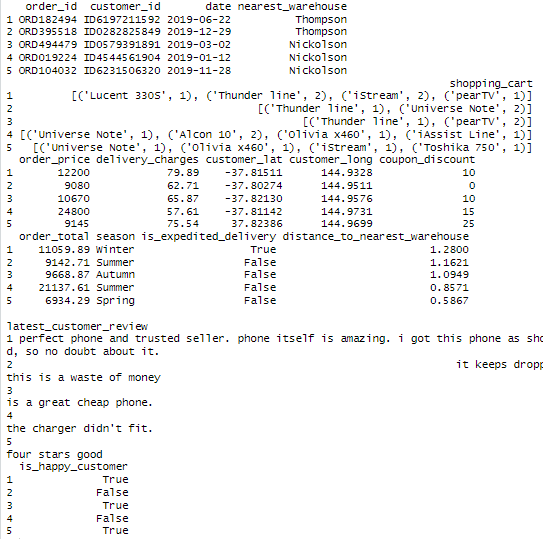
\includegraphics[width=0.6\textwidth]{graphics/Pre_processing_data/f8.PNG}
    \caption{Bảng dữ liệu thể hiện 5 dòng đầu tiên của mỗi biến}
    \label{fig:3.1}
\end{figure}

\begin{figure}[!htbp]
    \centering
    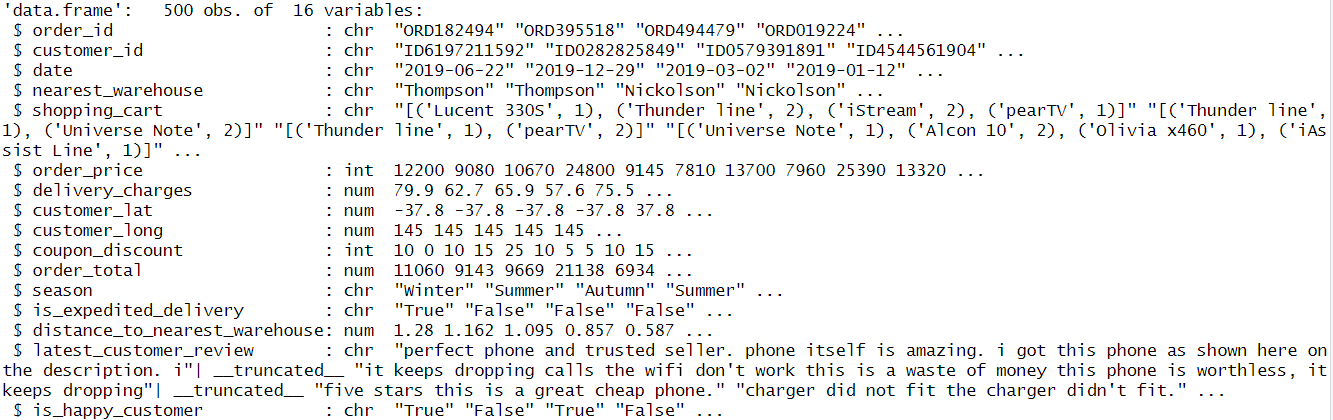
\includegraphics[width=1\textwidth]{graphics/Pre_processing_data/f9.PNG}
    \caption{Cấu trúc dữ liệu gốc của các biến}
    \label{fig:3.2}
\end{figure}
\subsection{Làm sạch dữ liệu}
Sau khi quan sát hình \ref{fig:3.2}, ta nhận thấy biến \textbf{date} đang có cấu trúc dữ liệu \textbf{chr}, không phù hợp với biến thời gian, và chưa thống nhất về định dạng (hình \ref{fig:3.3}). Bên cạnh đó, một số giá trị bị lỗi chính tả trong biến \textbf{season} và \textbf{nearest\_warehouse} (hình \ref{fig:3.4}).
\begin{figure}[!htbp]
    \centering
    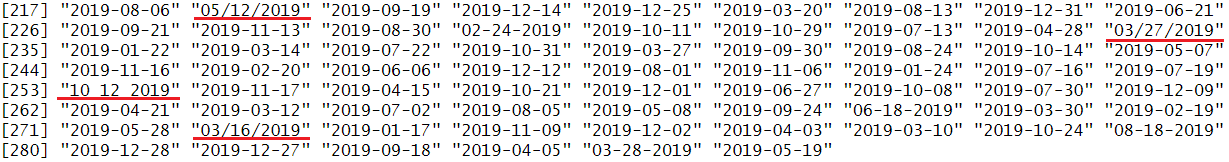
\includegraphics[width=1\textwidth]{graphics/Pre_processing_data/f10.PNG}
    \caption{Một số giá trị của biến \textbf{date} (được gạch chân) có định dạng lỗi}
    \label{fig:3.3}
\end{figure}

\begin{figure}[!htbp]
    \centering
    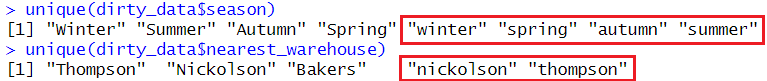
\includegraphics[width=0.7\textwidth]{graphics/Pre_processing_data/f11.PNG}
    \caption{Những giá trị bị lỗi chính tả trong biến \textbf{season} và biến \textbf{nearest\_warehouse}}
    \label{fig:3.4}
\end{figure}

% Ngoài ra, ta có thể dễ dàng thiết lập được công thức cho mối liên hệ giữa biến \textbf{order\_total} với các biến \textbf{order\_price}, \textbf{delivery\_charges} và \textbf{coupon\_discount}. Tương tự, ta cũng có công thức để tính khoảng cách từ khách hàng đến 3 kho hàng khác nhau, từ đó xác định được giá trị của \textbf{nearest\_warehouse} dựa vào kho hàng có khoảng cách ngắn nhất. Các biến này sẽ được tính toán lại bằng công thức để đối chiếu với giá trị thực tế.
\subsubsection{Điều chỉnh định dạng của biến date}
Chúng ta sẽ thực hiện việc chuẩn hóa và chuyển đổi biến \textbf{date} thành định dạng \textbf{``Date''} từ dữ liệu ban đầu để đảm bảo tính nhất quán trong phân tích. Thư viện \textbf{lubridate} sẽ được sử dụng vì nó cung cấp cho ta hàm \textbf{parse\_date\_time()} giúp phân tích và chuyển đổi các giá trị trong \textbf{dirty\_data\$date} về dạng thống nhất, dựa trên các mẫu định dạng được chỉ định trong \textbf{orders = c(``ymd", ``dmy", ``mdy")}. Sau đó, sử dụng hàm \textbf{as.Date()} để đưa giá trị về định dạng \textbf{``Date''}. Kết quả cho 10 giá trị đầu tiên có được biểu diễn trong hình \ref{f2}
\begin{figure}[!htbp]
    \centering
    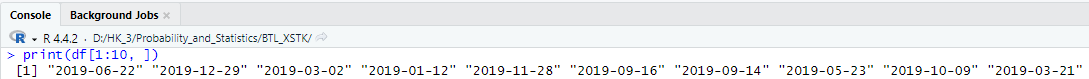
\includegraphics[width=\textwidth]{graphics/Pre_processing_data/f2.PNG}
    \caption{10 giá trị đầu tiên của biến \textbf{date} sau khi được sửa}
    \label{f2}
\end{figure} 
\subsubsection{Điều chỉnh định dạng biến season}
Ta sẽ tiến hành chỉnh sửa lại biến \textbf{season} dựa trên biến \textbf{date}. Biến \textbf{sum} được khởi tạo và được gán giá trị của <ngày trong tháng> + <tháng>\times100. Như vậy, tùy vào giá trị của \textbf{sum} mà ta sẽ xác định mùa tương ứng: Nếu \textbf{sum} nằm trong khoảng từ 301 (1 tháng 3) đến 530 (30 tháng 5), mùa được gán là Autumn (mùa thu); nếu \textbf{sum} nằm trong khoảng từ 601 (1 tháng 6) đến 831 (31 tháng 8), mùa là Winter (mùa đông); nếu \textbf{sum} nằm trong khoảng từ 901 (1 tháng 9) đến 1130 (30 tháng 11), mùa là Spring (mùa xuân); các giá trị còn lại (như từ 1 tháng 1 đến 28/29 tháng 2, hoặc tháng 12) được gán là Summer (mùa hè). (Ví dụ: Nếu ngày là 15/03, thì sum = 15 + 3 \times 100 = 315 và \textbf{season} được gán giá trị Autumn). Hình \ref{f3} thể hiện 10 giá trị của \textbf{season} trước và sau khi được sửa.
\begin{figure}[!htbp]
    \centering
    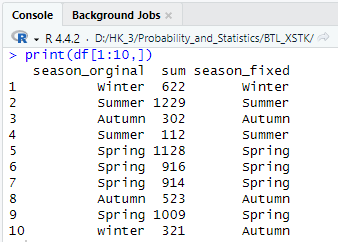
\includegraphics[width=0.4\textwidth]{graphics/Pre_processing_data/f3.PNG}
    \caption{Biến \textbf{season} trước và sau khi được tinh chỉnh}
    \label{f3}
\end{figure}

\subsubsection{Điều chỉnh tên kho hàng trong biến nearest\_warehouse}

Ta tiến hành việc chuẩn hóa dữ liệu trong biến nearest\_warehouse của tập dữ liệu dirty\_data bằng cách chuyển đổi tất cả các tên (``Thompson'', ``Nickolson'',  ``Bakers'') thành dạng Title Case (chữ cái đầu viết hoa). Thư viện \textbf{stringr} cung cấp hàm \textbf{str\_to\_title} dùng để chuyển đổi chuỗi ký tự sang dạng Title Case. Mục đích của việc chuẩn hóa định dạng văn bản này là để tăng tính nhất quán trong dữ liệu và cải thiện tính dễ đọc khi hiển thị hoặc sử dụng trong các báo cáo, phân tích. Hình \ref{f4} cho thấy hàm \textbf{unique()} được dùng để kiểm chứng việc định dạng lại dữ liệu.
\begin{figure}[!htbp]
    \centering
    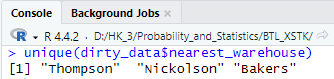
\includegraphics[width=0.4\textwidth]{graphics/Pre_processing_data/f4.PNG}
    \caption{Sử dụng hàm \textbf{unique()} để kiểm chứng kết quả}
    \label{f4}
\end{figure}

% \subsubsection{Kiểm tra giá trị trong biến order\_total}
% Ta sẽ tiến hành thực hiện các bước để tính toán lại tổng chi phí (\textbf{order\_total}) của các đơn hàng dựa trên các yếu tố liên quan (\textbf{order\_price}, \textbf{delivery\_charges}, \textbf{coupon\_discount}) và kiểm tra xem có sự khác biệt nào so với dữ liệu gốc hay không. Tổng chi phí đơn hàng được tính theo công thức \textbf{calculated\_order\_total} = \textbf{order\_price} \times (1 - \textbf{coupon\_discount}/100) + \textbf{delivery\_charges}. Công thức này áp dụng giảm giá (dựa trên phần trăm \textbf{coupon\_discount}) và cộng phí giao hàng (\textbf{delivery\_charges}) để tính tổng chi phí thực tế. Việc tính lại tổng chi phí đơn hàng là để kiểm tra giá trị của biến \textbf{order\_total} có sự sai lệch giữa công thức toán học và dữ liệu có từ thực tế hay không. Hình \ref{f5} biểu diễn một vài giá trị ban đầu của dữ liệu bị sai và giá trị được tính toán chính xác từ công thức.
% \begin{figure}[!htbp]
%     \centering
%     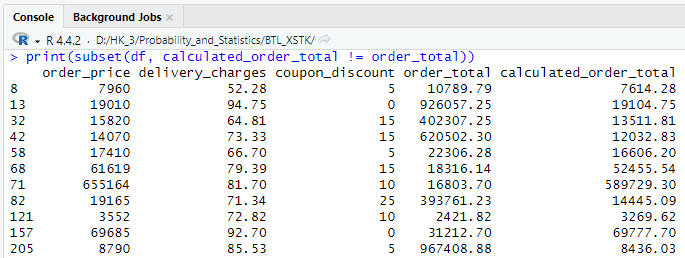
\includegraphics[width=0.7\textwidth]{graphics/Pre_processing_data/f5.PNG}
%     \caption{Giá trị gốc bị lỗi của \textbf{order\_total}} được cập nhật bởi giá trị mới từ \textbf{calculated\_order\_total} 
%     \label{f5}
% \end{figure}

% \subsubsection{Kiểm tra giá trị trong biến nearest\_warehouse}
% Ta sẽ sử dụng công thức Haversine (được trình bày trong phần \ref{Kien thuc nen}) để tính khoảng cách giữa hai điểm dựa trên tọa độ vĩ độ và kinh độ, sử dụng bán kính Trái Đất là 6371 km. Công thức được áp dụng để đo khoảng cách theo đường cong bề mặt Trái Đất, phù hợp cho dữ liệu địa lý. Hàm \textbf{haversine\_distance()} được thiết kế để tính khoảng cách từ khách hàng đến mỗi kho hàng, với đầu vào là tọa độ khách hàng và tọa độ nhà kho, hàm trả về khoảng cách giữa hai tọa độ trên. Sau khi hoàn tất việc tính khoảng cách từ một khách hàng bất kỳ đến cả 3 kho hàng, hàm \textbf{pmin()} được dùng để chọn ra kho hàng gần nhất và gán vào \textbf{distance\_to\_nearest\_warehouse\_fixed}. Hình \ref{f6} cho thấy một vài giá trị khoảng cách được tính lại có độ sai lệch bất thường so với giá trị gốc. Nếu quan sát kỹ, ta sẽ phát hiện giá trị \textbf{customer\_lat} tương ứng với những khoảng cách này xấp xỉ 37 trong khi hầu hết các giá trị cùng loại khác xấp xỉ -37. Điều này dẫn đến kết luận có sự sai sót (thiếu dấu âm) trong khâu nhập dữ liệu. Vì thế, ta quyết định sẽ thêm dấu âm cho các giá trị lỗi đã đề cập. Hình \ref{f7} liệt kê tất cả các giá trị của \textbf{nearest\_warehouse} bị lỗi được cập nhật lại, số lượng các giá trị lỗi này được giảm đáng kể, chứng tỏ kết luận trên là đúng đắn.
% \begin{figure}[!htbp]
%     \centering
%     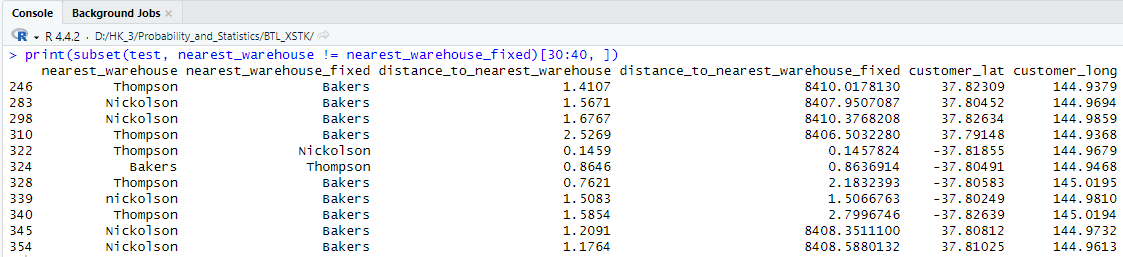
\includegraphics[width=\textwidth]{graphics/Pre_processing_data/f6.PNG}
%     \caption{Một vài giá trị khoảng cách gốc và giá trị khoảng cách được tính lại}
%     \label{f6}
% \end{figure}
% \begin{figure}[!htbp]
%     \centering
%     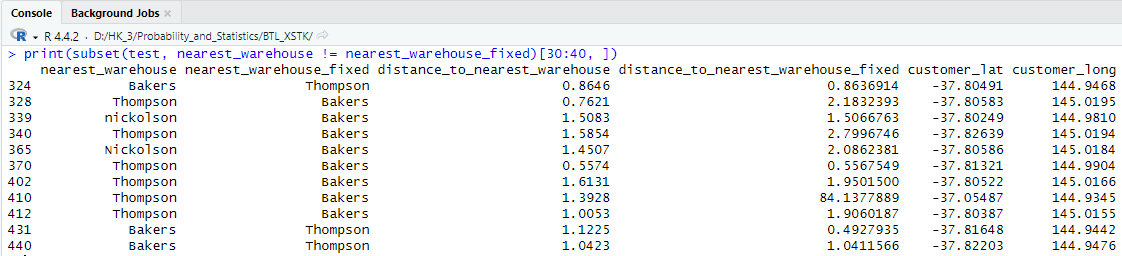
\includegraphics[width=\textwidth]{graphics/Pre_processing_data/f7.PNG}
%     \caption{Các giá trị \textbf{nearest\_warehouse} lỗi được cập nhật}
%     \label{f7}
% \end{figure}

% Như vậy, có sự sai lệch giữa giá trị được áp dụng công thức toán học và giá trị được đo đạc từ thực tế. Điều này có thể là do ảnh hưởng của các yếu tố ngẫu nhiên và chúng sẽ được phân tích ở các phần sau.